\documentclass[12pt]{article}
\usepackage[utf8]{inputenc}
\usepackage{amsmath}
\usepackage{graphicx}
\usepackage{amsfonts}
\usepackage{adjustbox}
\usepackage{listings}
\usepackage{color}
\usepackage{braket}
\usepackage{pgfgantt}
\usepackage{subcaption}
\usepackage{tabularx}
\usepackage{pdfpages}
\usepackage{verbatim}
\usepackage[table,xcdraw]{xcolor}

\definecolor{dkgreen}{rgb}{0,0.6,0}
\definecolor{gray}{rgb}{0.5,0.5,0.5}
\definecolor{mauve}{rgb}{0.58,0,0.82}

\graphicspath{{figures}}

\usepackage{geometry}
 \geometry{
 a4paper,
 total={170mm,257mm},
 left=25mm,
 right = 25mm,
 top=30mm,
 bottom=35mm
 }

\newcommand{\detailtexcount}[1]{%
  \immediate\write18{texcount -merge #1.tex > #1.wcdetail }%
  \verbatiminput{#1.wcdetail}%
}

\newcommand{\newp}
    {
    \vskip 0.5cm 
  }

\newlength\tindent
\setlength{\tindent}{\parindent}
\setlength{\parindent}{0pt}
\renewcommand{\indent}{\hspace*{\tindent}}

\usepackage[backend=biber]{biblatex}

\addbibresource{diss.bib}

\numberwithin{equation}{section}

\nocite{*}

\lstset{frame=tb,
  language=Python,
  aboveskip=3mm,
  belowskip=3mm,
  showstringspaces=false,
  columns=flexible,
  basicstyle={\small\ttfamily},  numbers=none,
  numberstyle=\tiny\color{gray},
  keywordstyle=\color{blue},
  commentstyle=\color{dkgreen},
  stringstyle=\color{mauve},
  breaklines=true,
  breakatwhitespace=true,
  tabsize=3
}


%TC:ignore
\title{Analysis of the Quantum Advantages for Deep Hedging}

%TC:endignore

\author{Soham Deshpande\\Supervisor: Dr. Srinandan Dasmahapatra
\\Second Supervisor: Dr. Hansung Kim}
\date{April 2025}

\begin{document}

\maketitle
\vspace{10cm}
\begin{centering}
A project report submitted for the award of MEng Computer Science
\end{centering}
\thispagestyle{empty}

%TC:ignore
%\detailtexcount{progress}
%TC:endignore






\clearpage

\pagenumbering{roman}

%TC:ignore
\begin{abstract}
Parameterised Quantum Circuits (PQCs) have opened many doors, one 
such being the use in financial markets. In this paper, I look at the problem 
of developing an accurate market generator through the use of quantum computing
for the purposes of hedging. 
Given a Quantum Circuit Born Machine (QCBM), we are able to exploit the high 
expressibility to generate synthetic 
data that mimics the statistical distribution of the original dataset. The market 
generator is then used to simulate an 
underlying asset to maturity with the intent of learning an optimal hedging strategy 
$\pi^*$, a showcase of a data-driven approach to hedging exposure. I show that 
the synthetic 
data produced by this method has shown to capture the fat tails of the market 
better than classical methods, as well as demonstrating superiority in 
out-of-sample testing with COVID data. Different generator 
architectures have been compared to maximise the quality of the synthetic data 
and avoid issues with barren plateaus. 
The findings of 
this research will contribute to the growing literature on risk management in 
quantitative finance, with applications of the market generator extending beyond 
deep hedging. 
\end{abstract}

\clearpage


\tableofcontents
%TC:endignore
\clearpage



\pagenumbering{arabic}


\section{Problem Statement}
The problem of hedging a portfolio of derivatives is an important part of 
risk management used widely in financial institutions. This involves understanding 
the exposure to the market, and taking strategic positions to negate some of this 
risk. In an ideal world we can picture a perfect, 
frictionless market where transaction costs are negligible and every asset in 
the space has a price; here we can price and hedge perfectly. Unfortunately in 
practice, we experience incomplete markets due to frictions, costs that interfere 
with trades such as transaction costs or imperfect information. In addition, recent 
years have presented markets with periods of heightened volatility, much that disobey 
traditional frameworks. This generates the need for complex, realistic market 
models that can account for these.
\newp
Traditional methods of hedging options has shown to be ineffective for equity 
markets, new information resulting in rapid changes. Much of the available 
literature models the market as a smooth, continuous stochastic process within 
a Gaussian space. Such models are sufficient for common market activity but fail 
when presented with discontinuous moves in price. These can be reactions to 
geopolitical events or natural disasters; traditional
models are incapable of capturing the effects. The introduction of Jump-diffusion 
models aimed to solve this issue though face similar issues. In reaction, we have 
recently observed non-parametric models that harness neural networks and machine 
learning which aim to demonstrate high accuracy on out-of-sample forecasts.
\newp
An alternative approach that has recently emerged utilises the power of 
quantum computing. The introduction of parameterised quantum circuits(PQCs) have 
opened up new pathways for navigating complex, large scale time series datasets. 
Through rotation gates and quantum entanglement, we are able to learn complex 
distributions and relationships. 
\newp
In this research, I aim to tackle the problem 
of generating synthetic financial data, addressing issues that come about from 
using a classical method particularly the estimation of tail risk and skewness. 
Through comparisons between traditional approaches, 
I aim to demonstrate an advantage in the expressibility of Quantum Circuit Born 
Machines (QCBMs); these will be described quantitatively using measures such as 
Value at Risk (VaR) and Conditional Value at Risk (CVaR). By performing out-of-sample 
tests on COVID and Oil data, I aim to highlight the weaknesses of traditional models 
and showcase a quantum superiority.
There will also be an exploration into the variety of architectures 
available for the QCBM, evaluating different ansatz designs. Where unusual behaviours
due to quantum physics occur, such as barren plateau, I will explore in greater detail 
as well as any circuit optimisation techniques that may present themselves as 
possible solutions. 
\newp
This paper will aim to add to the existing literature on risk management for 
financial firms as well as providing a framework for generating synthetic 
data. In addition to that, I aim to extend to the QCBM research that exists 
currently, noting down any behaviours that may be of interest to the curious 
and potential 
experts in the field. 
\clearpage
\subsection{Aims \& Goals}
This section aims to provide a high-level insight into the goals of the 
project with more detailed explanations being left for their respective sections. 
\newp 
Market data, though appearing entirely stochastic at first glance, contains many 
hidden patterns and relationships. Classical methods such as Black-Scholes  
\autocite{blackscholes} have been proposed to capture some of this behaviour, 
though built on unrealistic assumptions, these govern 
our fundamental understanding of quantitative finance. With the move to the new era 
of electronic trading, the need for more complex markets models became more present.
Being able to trade within nanoseconds presented traders with a new, human-free method 
of trading, moving to a purely mathematical approach. In this approach we strive
for optimal strategies to make money, taking calculated positions and limiting 
exposure to large market movements. It is here where traditional methods started 
to be insufficient; particua
\clearpage 


\section{Related Literature}
To place this research within the context of existing literature, we can split 
the project into 2 components: the market generator, and 
parameterised quantum circuits.
\newp
The work around deep hedging has evolved, moving away from 
Greek-based hedging towards a sturdier framework using machine 
learning. Here a lot of work is being done, with many papers emphasising 
on using neural networks for optimising delta and gamma exposure
\autocite{armstrong_deep_2024,qiao_enhancing_2024}.
Buehler introduced an approach, modelling trading decisions 
as neural networks instead of relying on parameterised models
\autocite{buehler_deep_2019}. Subsequent advancements focussed on developing 
realistic market simulators. Wissel 
proposed a market model for path generation of options but this still 
employed risk-neutral diffusion\autocite{schweizer_arbitrage-free_2008}. Wiese 
then introduced 
a new dimension by using GANs to convert options into 
local volatility models with simpler no-arbitrage constraints. This focussed 
on the local stochastic nature of options
\autocite{choudhary_funvol_2023,wiese_deep_2019,wiese_multi-asset_2021}.
Some approaches suggest using actor-critic reinforcement learning algorithms to 
solve for an optimal value function, a move towards searching for a global
maximum over local risk management
\autocite{buehler_deep_2022,movahed_introducing_2024}.
\newp
Recent research explores using quantum computing to 
hedge portfolios, here the authors presented a quantum reinforcement learning 
method based on policy-search and distributional actor-critic algorithms. 
They proposed using a Quantum Neural Network to approximate the value of a 
given value function by predicting the expected utility of returns using compound 
and orthogonal layers which were built using Hamming-weight
unitaries \autocite{kerenidis_classical_2022}. 
\newp TO CHANGE:
This helped overcome the barren 
plateau by ensuring the gradient 
variance does not vanish exponentially with qubit count. 
\newp
Another method models 
the entire return distribution, leveraging parameterised circuits to learn categorical 
distributions and capture variability and tail risk 
\autocite{cherrat_quantum_2023,dasgupta_loading_2022}.
\newp
There is an immense amount of research being done on exploiting the benefits of 
quantum computing, recent advancements being in quantum algorithms. 
These claim to provide exponential speed-up over classical 
methods, though in reality, we see great complexity in state preparation, requiring 
$\Theta(2^n/n)$ circuit depth with n qubits or $\Theta(n)$ circuit depth with 
$\Theta(2^n)$ ancillary qubits\autocite{zhang_quantum_2022}. Here we see hybrid 
models such as Born machines
and Quantum generative adversarial networks boasting high generalisation ability
\autocite{ganguly_implementing_nodate,gili_2022_do,horowitz_quantum_2022}.
\newp
There has also been research in harnessing back action from quantum weak 
measurements to enhance the ability of quantum machine learning algorithms. 
In quantum reservoir computing,
the ability to retain information from past inputs plays a key role in processing 
temporal series and producing future predictions
\autocite{franceschetto_harnessing_2024,fujii_quantum_2020,garcia-beni_squeezing_2024,mujal_time-series_2023}.
\newp
This research aims to combine the needs of financial firms in hedging portfolios
using realistic market models by utilising QCBMs as a tool 
for simulating paths in combination with deep hedging engines for learning 
optimal policies. A comparison will be made against hedging under Merton-Jump 
diffusion. 
\clearpage
\section{Markets and Derivatives}
The market, though inherently can be thought of as a completely random process,
where bids and asks are fulfilled, can be modelled as a stochastic process. The 
aim of this chapter is to serve as a brief introduction and set up notation for 
later chapters. \\
\subsection{Market}
Consider a market with a finite time horizon $T$ defined on the probability space 
($\Omega,\mathcal{F},P$) along with a filtration $\bold{F} = \{\mathcal{F}| 0 \leq t \leq T \}$ 
This can be thought of as an adapted (n+1) dimensional It\^{o} process 
$X(t) = (X_0(t), X_1(t),...,X_n(t))$
which has the form 
\begin{equation}
dX_0(t) = \rho(t,\omega)X_0(t)dt;\hspace{8pt}X_0(0)=1
\end{equation}and
\begin{equation}
dX_i = \mu_i(t,\omega)dt+\sigma_i(t,\omega)dB(t);\hspace{8pt}X_i(0)=x_i 
\end{equation}
where $X_i(t)$ as the price of asset $i$ at a given time $t$.
\\
We can define a portfolio in the market as 
\begin{equation}
\theta(t,\omega) = (\theta_0(t,\omega),\theta_1(t,\omega),...,\theta_n(t,\omega))
\end{equation}
where the components $\theta_n(t,\omega)$ represents the number of units of a given 
asset held at time $t$.\\
Following from that, we can define the value of a given portfolio to be 
\begin{equation}
  V(t,\omega) = V^{\theta}(t,\omega) = \sum_{i=0}^n \theta_i(t)X_i(t)
\end{equation}
Lastly, it is important to state that the portfolio is self-financing, any 
trading strategy $\alpha$ requires no extra cost beyond the initial capital
\begin{equation}
  V(t) = V(0) + \int_0^t\theta(s)\cdot dX(t)
\end{equation}
We can also make the following assumptions about the market:
\begin{itemize}
  \item The market is liquid, allowing the trade to execute instantaneously
  \item There is no bid-ask spread, the price to buy and sell is the same 
  \item Trading actions taken have no impact on the price of the asset traded 
\end{itemize}


\subsection{Derivatives}
A derivative refers to any financial instrument whose value is derived from an 
underlying security, the most fundamental being futures and options. It is common 
practice to refer to the given underlying security as just 'underlying'.
\subsubsection{Futures}
A futures contract is a contract that gives the right and obligation to buy a 
given asset $i$ a specified time $T$ at price $K$. 
\subsubsection{Options}
The two types of options going to be explored are Puts and Calls; a Call option 
gives the owner the right but not the obligation to buy a given asset $i$ at 
a specified price $K$ at time $T$. Similar to the Call, a Put option gives the 
owner the right but not the obligation to sell a given asset $i$ at a price $K$ 
at time $T$. If the owner can exercise the option any time up to $T$, we call 
this an American option. For the purposes of this research, I will only be 
dealing with vanilla European options.\\ 
It is important to define the payoffs for both options: 
\begin{equation}
C_T = max(0,S_T-K)
\end{equation}
\begin{equation}
P_T = max(0,K-S_T)
\end{equation}



\subsection{Market Data}
In this research I will be focussing on hedging a portfolio consisting of a single 
asset, hence requiring a simulation of a single underlying.
\subsubsection{Euro Stoxx 50}
The Euro Stoxx 50 Index (SX5E) and relevant derivatives. This is a stock index of 50 stocks in the Eurozone. 
This index captures around 60\% of the free-float market capitalisation of the 
Euro Stoxx Total Market Index which covers about 95\% of the free-float market 
in the Eurozone\autocite{a2021_euro}. Rationale behind choosing this index is the availability of data,
options traded with SX5E as the underlying and the liquidity of the index.
\\
Derivatives that are held in the portfolio to be hedged will include those that 
have SX5E as the underlying, examples are weekly, monthly, and quarterly
expiration options. These are European-style so can only be exercised upon 
maturity. Data can be found on Bloomberg\autocite{bloomberg_2023_bloomberg} and Refinitiv
\autocite{lseg}.
\begin{figure}[h]
    \centering
    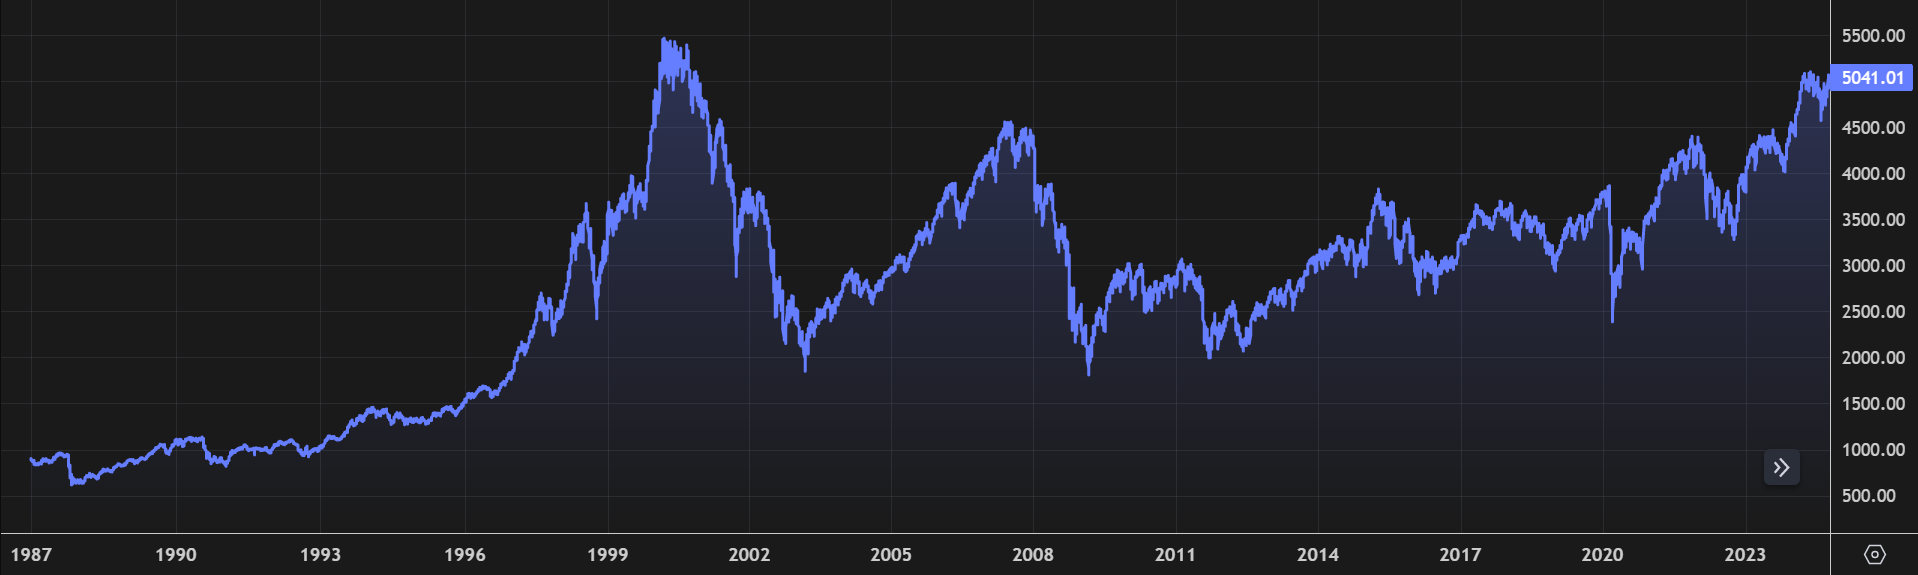
\includegraphics[scale=0.35]{sx5e.png}
    \caption{Euro Stoxx 50 price chart}
\end{figure}

\subsubsection{Brent Crude Oil}
It was appropriate to try and learn a volatile commodity. Sensitive to price 
movements.

\clearpage

\section{Merton-Jump Diffusion Model}
My model of choice for comparison is the Merton-Jump Diffusion model, this an 
elementary model that goes beyond Black-Scholes by trying to capture the negative
skewness and excess kurtosis of log price returns. This is done through the 
addition of a compound Poisson jump process. This aims to represent the jumps 
we observe in the market in a more realistic fashion rather than assuming constant 
volatility assumption made by Black-Scholes. As a simplification, I will be referring 
to Black-Scholes by BS and Merton-Jump Diffusion with MJD.
\subsection{Model}
A standard derivation of the model will allow us to explore its assumptions and 
limitations. This model consists of two components, jump and diffusion. The 
diffusion will be modelled using a Weiner process and log-normal jumps driven 
by a Poisson process. This gives us the following
SDE. 
\begin{equation}
  \italic{d}S_t = (\alpha - \lambda k)S_tdt + \sigma S_t dW_t + (y_t-1)S_tdN_t
\end{equation}
where $W_t \text{ and } N_t$ are Weiner and Poisson processes respectively. 
$\lambda$ represents the intensity of the jumps, $\alpha$ is the drift rate
(expected return), and $k$ is the expected jump size. 
Solving the equation gives us an exponential L\'{e}vy model described by 
\begin{equation}
  S_t = S_0e^{\mathcal{L}_t}
\end{equation}
where $S_t$ is the stock price at time t, $S_0$ is the initial stock price. 
We can also define $\mathcal{L}_t$ to be 
\begin{equation}
  \mathcal{L}_t = (\alpha - \frac{\sigma^2}{2}-\lambda k)t + \sigma W_t + 
  \sum^{N_t}_{i=1}Y_i
\end{equation}
\subsection{Assumptions \& Limitations}
Through inspection of the equations, we can observe the following assumptions:
\begin{enumerate}
\item The asset price experiences continuous, random fluctuations over time,
  governed by Brownian motion (GBM)
\item The asset price experiences sudden, discontinuous jumps modelled by a 
  Poisson process, occurring at a constant rate $\lambda$
\item Jumps sizes are assumed to be log-normal $ln(y_t) \sim \mathcal{N}(\mu,\sigma^2)$
\end{enumerate}
Starting with the first assumption, we can see that assuming GBM may produce
unrealistic behaviour, most important being a lack of excess kurtosis.
Markets 
often exhibit fat tails, especially within commodities. One such event may 
be the release of news from OPEC+, the organisation of petroleum-exporting 
countries. A restriction in oil production may cause the price of oil to jump 
rapidly. In recent times, wars and conflict has also become 
ever present, causing large movements in asset prices; therefore it is not 
unrealistic to
expect extreme price movements to be more frequent than can be modelled 
by a Gaussian.
\newp
The MJD requires calibration of parameters before use, typically done using historical 
data or implied volatility surfaces. Once calibrated these become assumptions of 
the data and so do not change even if the market observations move away from it. 
This would lead us to expect higher overfitting to the historical data, possibly 
failing in unseen conditions such as the market's reaction to COVID. 
\newp 
We also may expect poor volatility clustering with the MJD; constant volatility 
is not experienced by the market, instead periods of high volatility followed 
by periods of low volatility is observed. Though this paper won't be focussing 
on this phenomenon, it is important to consider.
\subsection{Calibration}
In this research, I have chosen to use maximum likelihood estimation to estimate 
the parameters for the MJD model. In the analytical solution we require five 
parameters: $\alpha$, $\sigma$, $\mu_j$, $\delta$, and $\lambda$. These are the 
expected return, volatility of the given asset, expectation of the jump size, 
standard deviation of the jump size and lastly the jump intensity. We can then 
use MLE on the probability density of log returns $S_t = ln(\frac{S_t}{S_0})$ 
\begin{equation}
P(S_t) = \sum^\infty_{i=0} \frac{e^{-\lambda t}(\lambda t)^i}{i!}N(S_t;(\alpha - 
\frac{\sigma^2}{2}-\lambda k)t+i\mu_j,\sigma^2t+i\delta^2)
\end{equation}
The likelihood function hence becomes 
\begin{equation}
  L(\theta;S) = \prod^T_{t=1}P(S_t)
\end{equation}
We can minimise the negative log-likelihood to obtain 
\begin{equation}
  -\ln L(\theta;S) = -\sum^T_{t=1}\ln P(S_t)
\end{equation}
Another popular option to calibrate the MJD model is by considering the implied 
volatility surface of existing options.







\clearpage

\section{Parameterised Quantum Circuits}

\subsection{Parameterised Circuits}
Consider a set of unitaries... 
\subsection{Born Rule}
An essential part of quantum computing involves the existence of the Born
Rule. Born's measurement rule states that:
\begin{equation}
p(x) = |\langle x|\psi(\theta)\rangle|^2
\end{equation} where 
\begin{equation}
|\psi(\theta)\rangle = U(\theta)|0\rangle^{\otimes n}
\end{equation}
The state $|\psi(\theta)\rangle$ is generated by evolving state $|0\rangle$
according to a Hamiltonian $H$ that is constructed from gates. Once combined, the 
gates form a parameterised quantum circuit which is parameterised by using the 
variables governing each gate, $\theta$. By tuning the values of $\theta_i$ one 
can allow for an evolution to any state that will serve as a solution to a given 
problem. \\ 
By taking the distribution associated to the state, $|\psi(\theta)\rangle$ we can 
treat the PQC as a generative model, upon measurement will 
generate samples of a target distribution $\chi$. This model is parameterised 
by $\theta$, which defines a quantum circuit $U(\theta)$ made up of a set of quantum 
gates.
By measuring the circuit, we can obtain samples. Producing samples that emulate 
the target distribution involves minimising the parameters of the circuit $U(\theta)$, 
a process once convergence is reached, will generate accurate samples 
\cite{liu_differentiable_2018}.

\subsection{State Preparation}
We require state preparation to transfer the classical data onto the 
Hilbert space. This involves a function $\phi$ that maps the input vector to 
an output label. There are many encoding schemes, each of which aim to offer 
high information density and low error rates; main methods include: basis, amplitude, angle encoding, and QRAM. 
\\
Without the use of ancillary qubits, we can expect an exponential circuit depth
to prepare an arbitrary quantum state. Using them we can reduce the depth to be 
sub-exponential scaling, with recent advancements reaching $\Theta(n)$ given $O(n^2)$
ancillary qubits
\cite{shaib_efficient_2023,zhang_quantum_2022}.




\subsection{Measurements}
In quantum mechanics, we can define measurement to be any process that probes a 
given quantum system to obtain information, we may also refer to this process as 
a measurement in the computational basis when focussing on quantum information 
science. Let's consider a quantum state 
$|\psi \rangle = \alpha_0|0\rangle+\alpha_1|1\rangle$ which gives us $|0\rangle$
with probability $|\alpha_0|^2$ and $|1\rangle$ with probability $|\alpha_1|^2$. 
If measured in the standard basis we would expect the outcome to be $|k\rangle$
with a given probability. This outcome would result in the output 
state of the measurement gate to also be $|k\rangle$, resulting in the original 
state $|\psi\rangle$ to be irreversibly lost. We can refer to this as a collapse of state. 

\clearpage
\section{Quantum Circuit Born Machine}
Given a dataset $D = \{x_1, x_2.. x_n\}$ consisting of n samples and obeys a 
given distribution $\chi_d$, we would like the QCBM to learn the distribution 
and generate synthetic data points that are of the distribution $\chi_s$ such that
$\chi_s$ approximates $\chi_d$.
The QCBM is a subclass of parameterised quantum circuits, 
here the quantum circuit contains parameters which are updated during a training 
process. The QCBM takes the product state $\ket{0}$ as an input, and through an 
evolution, transforms into a final state $\ket{\phi_0}$ by a sequence of unitary 
gates. This can then be measured to obtain a sample of bits 
$x \sim p_\theta (x_s)=|\bra{x}\ket{\phi_\theta}|^2$ . By training the model we 
are aiming to let $p_\theta$ approach $\chi_d$. 
\\
The ansatz for this quantum circuit consists of 7 layers
of 1-qubit gates with entangling layers in between them. These are 
entangled using the CNOT gates as found in the appendix. The number of wires 
needed depends on the precision required for the generated data. The estimated
precision is 12-bit, so the samples are able to take $2^{12}$ different values in 
the range of $ (v_{min} - \epsilon, v_{max} + \epsilon )$, where $\epsilon > 0 $
allows data to be generated that lie outside the range $(v_{min},v_{max})$ of the 
original data.
\\
The QCBM takes a $n \times m$ matrix of parameters in the range $(-\pi, \pi)$ as 
input, in the form of a dictionary. Each angle takes one of $2^k$ discrete values, 
where $k$ is a model parameter. The resulting space therefore spans to: 
$(2^m)^{n\cdot m}$.


\subsection{Architectures}
\subsubsection{Brick}
\subsubsection{Pyramid}
\subsubsection{Butterfly}

\subsection{Barren Plateau}
A point of concern when searching for the optimal set of $\theta s$ is the large 
search space, here we may observe issues such as barren plateau(BP). BP 
insists that the gradient of the parameters of a given PQC will vanish exponentially 
w.r.t the search space.
\\ 
Introduce proof of $\frac{\partial C}{\partial \theta} \rightarrow 0 $


\subsection{ZX Calculus}
ZX Calculus as a method to optimise/minimise t gate count. introduce what a 
non clifford gate is.



\section{Results}

\subsection{Path Generation}
\subsubsection{VaR \& CVaR}
\subsection{Hedging}

\subsection{Barren Plateau}

\subsubsection{ZX Calculus}

\clearpage 

\section{Outlook and Conclusions}


\clearpage
\section{Appendix}
\subsection{QCBM Architectures}

\begin{figure}[h]
    \centering
    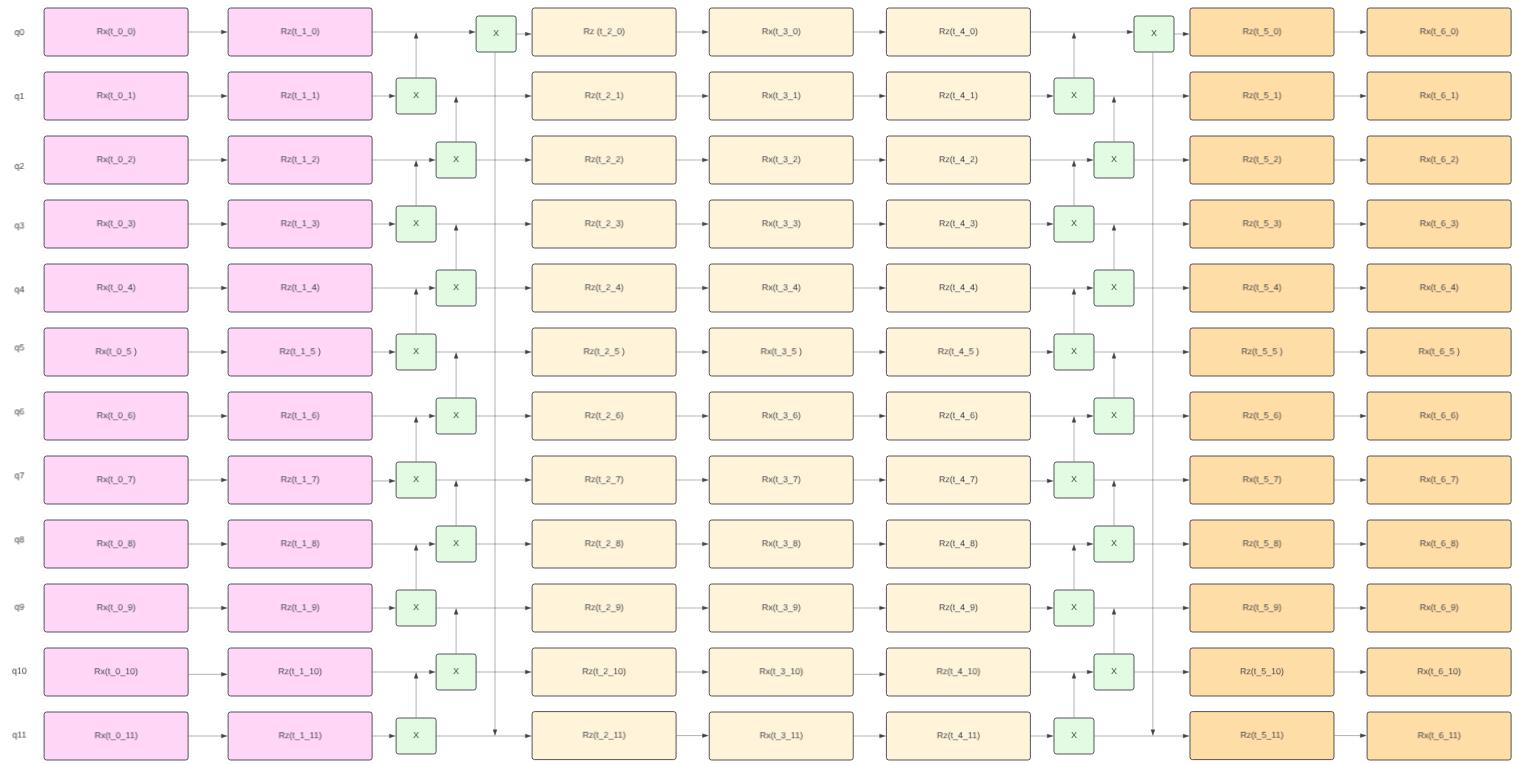
\includegraphics[scale=0.3, angle=270, width=\textwidth-209]{qcbm1.png}
    \caption{QCBM architecture}
\end{figure}
\clearpage


\printbibliography

\end{document}

